
\documentclass[letter,12pt]{article} 

\usepackage[top = 5cm, bottom = 2.5cm, left = 2.5cm, right = 2.5cm]{geometry}  
\usepackage[T1]{fontenc}
\usepackage[utf8]{inputenc}
\usepackage[spanish,es-tabla]{babel}
\spanishdecimal{.}
\usepackage{multirow} 
\usepackage{booktabs} 
\usepackage{graphicx} 
\usepackage{epstopdf}
\usepackage{setspace}
\setlength{\parindent}{0in}
\usepackage{float}
\usepackage{fancyhdr}
\usepackage{amsmath,mathtools}
\usepackage{amsfonts}
\usepackage{amssymb}
\usepackage{xcolor}
\usepackage{pdfpages}
\usepackage{apacite}
\usepackage{subfig}


\pagestyle{fancy} 

\fancyhf{} 

\lhead{\footnotesize  Proyecto } 	
\rhead{\footnotesize Gallardo Tinoco} 

\cfoot{\footnotesize \thepage} 	


\begin{document}
\begin{titlepage}
	
	\begin{center}
		\vspace*{-1in}

		
		UNIVERSIDAD NACIONAL AUTONOMA DE MEXICO\\
		\vspace*{0.15in}
		FACULTAD DE INGENIERÍA \\
		\vspace*{0.15in}
		INGENIERÍA EN COMPUTACIÓN \\
		\vspace*{0.6in}
		\begin{large}
			Laboratorio de Computación Grafica E Interacción Humano-Computadoras\\
		\end{large}
		\vspace*{0.1in}
		\rule{160mm}{0.1mm}\\
		\vspace*{0.1in}
		\begin{large}
			Grupo: 11\\
			Grupo de teoría: 3\\
			Semestre 2021-2\\
		\end{large}
		\vspace*{0.2in}
		\begin{Large}
			\textbf{Proyecto } \\
		\end{Large}
		\vspace*{0.2in}
		\begin{large}
			Fecha de entrega limite: 25 de julio de 2021\\
		\end{large}
		\vspace*{0.3in}
		\rule{80mm}{0.1mm}\\
		\vspace*{0.1in}
		\begin{large}
			418046595 \\
			andrwe713@gmail.com \\
			Gallardo Tinoco Andrés Amadeus\\
		\end{large}
	\end{center}
	
\end{titlepage}
\newpage
\section{Desarrollo}
\subsection{Modelado}
\begin{figure}[H]
		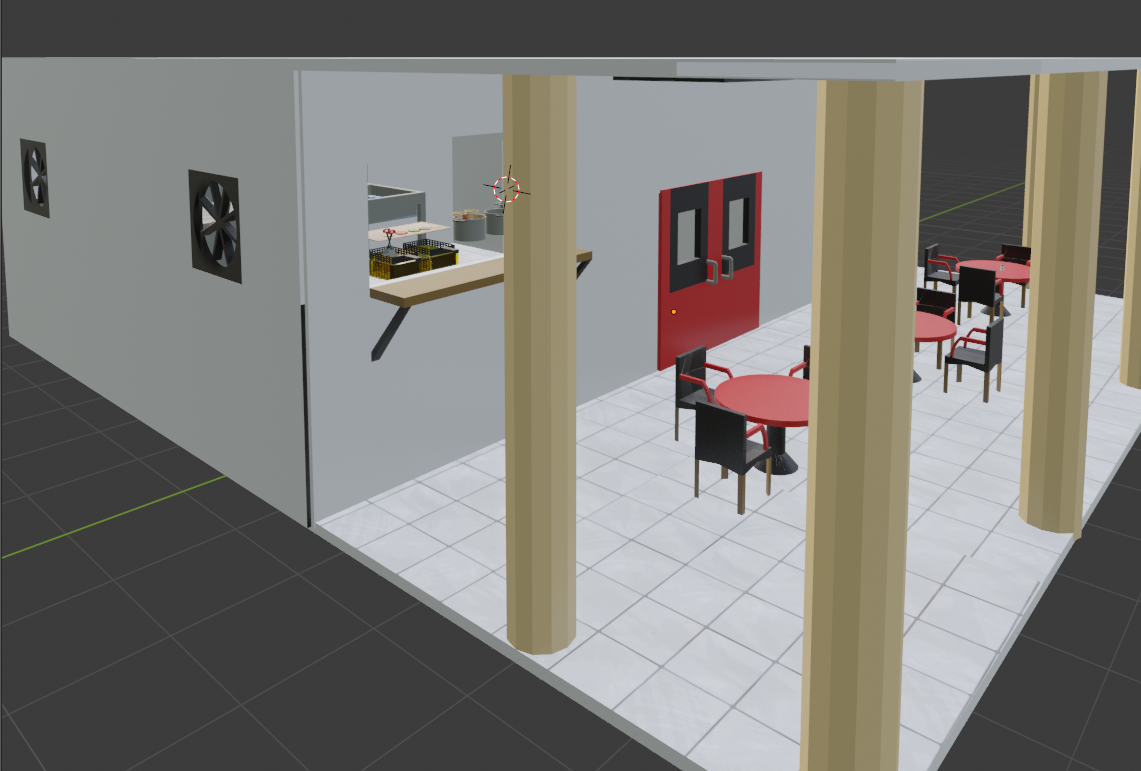
\includegraphics[scale=0.5]{img/img1}
		\centering
		\caption{Modelo en software Blender}
	\end{figure}
\begin{figure}[H]
		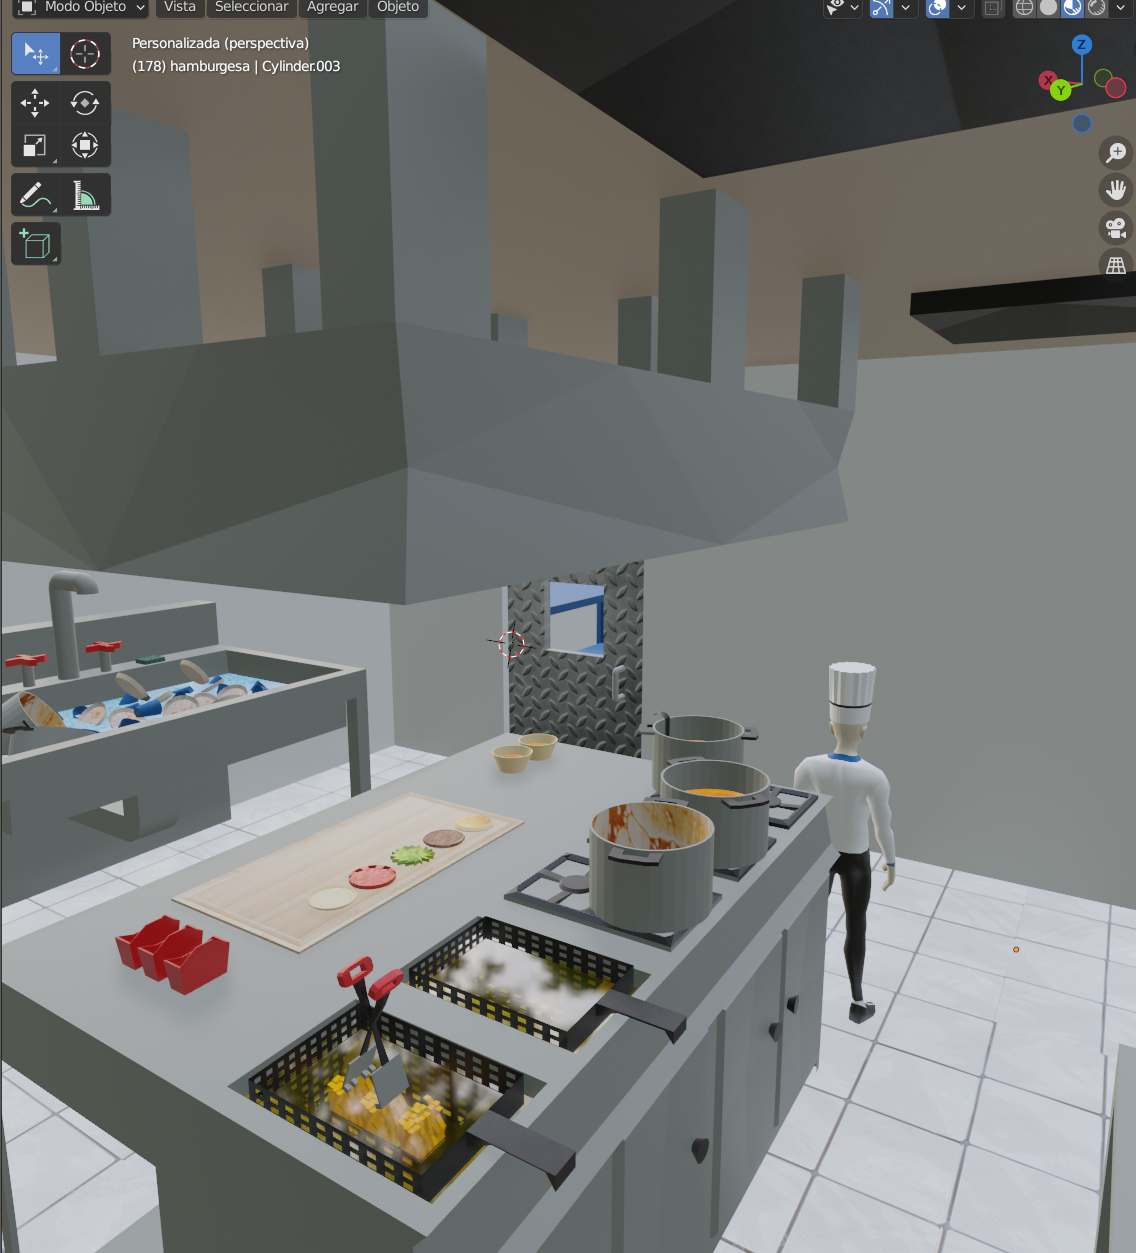
\includegraphics[scale=0.5]{img/img2}
		\centering
		\caption{Modelo en software Blender}
	\end{figure}

Todos los modelos son únicos y fueron realizados en el software de Blender, de igual forma fueron texturizados en dicho software, todos los modelos están en un solo archivo para manejar las dimensiones de estos, el archivo esta disponible en el repositorio de GitHub.\\

$https://github.com/AndresAmadeus/Proyecto\_compu\_grafica$\\


\subsection{Importacion}
\begin{figure}[H]
		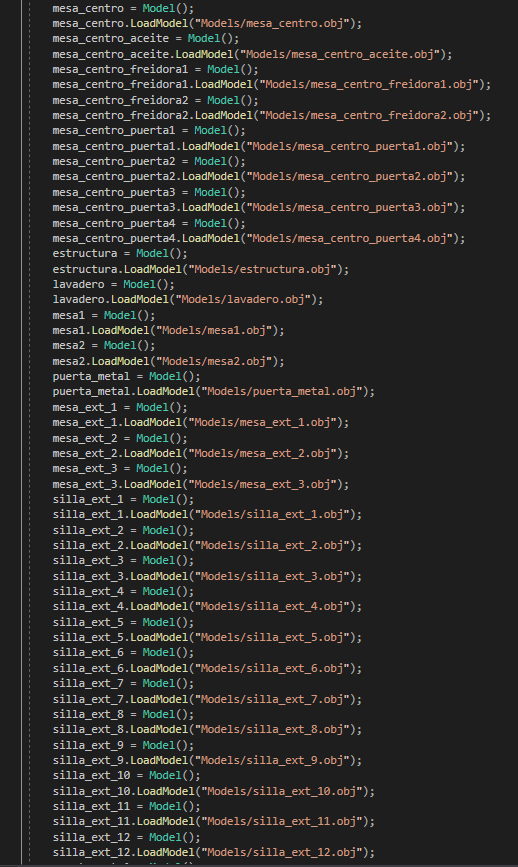
\includegraphics[scale=0.5]{img/img3}
		\centering
		\caption{Codigo}
	\end{figure}
\begin{figure}[H]
		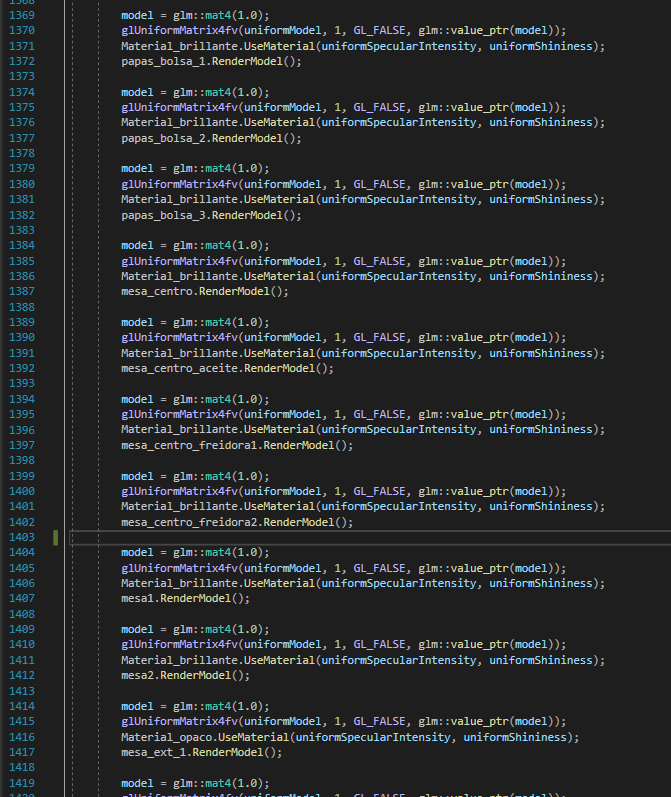
\includegraphics[scale=0.4]{img/img4}
		\centering
		\caption{Codigo}
	\end{figure}
\begin{figure}[H]
		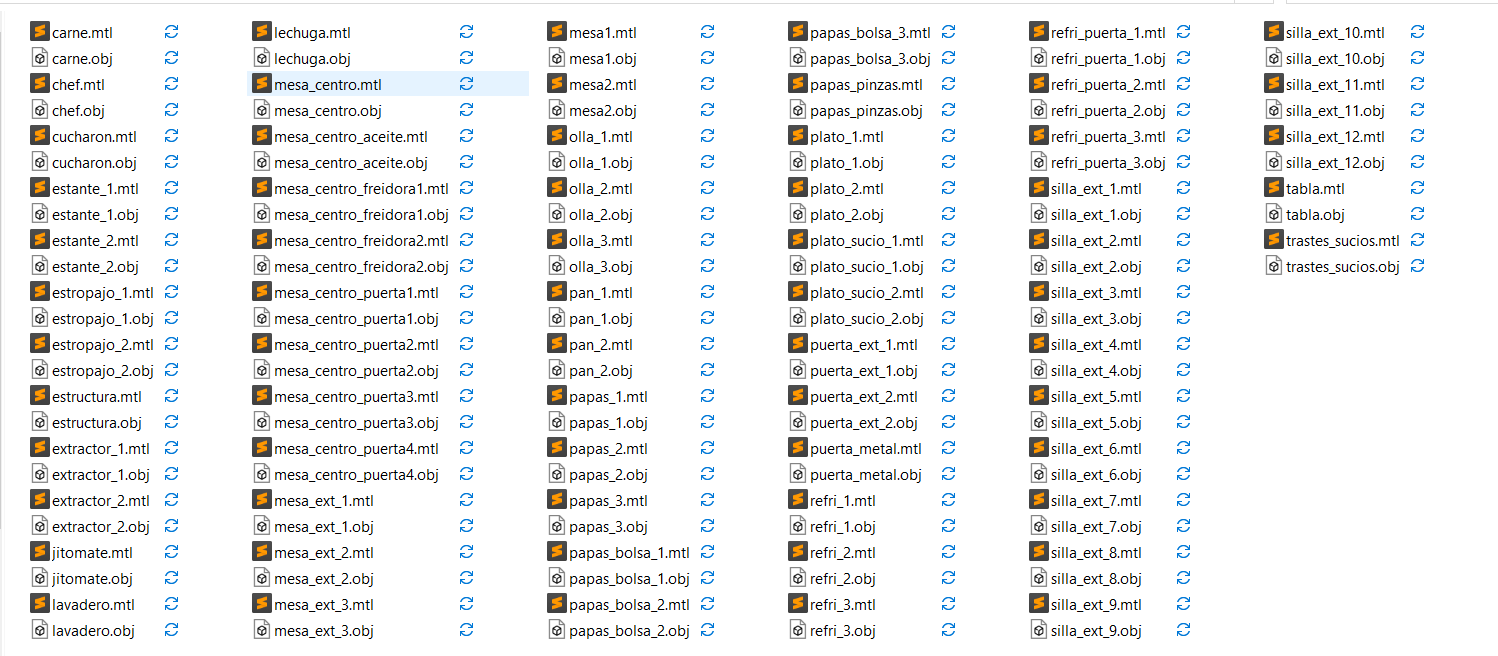
\includegraphics[scale=0.5]{img/img5}
		\centering
		\caption{Modelos}
	\end{figure}

Carga de todos los modelos, con un total de 65 modelos, (varios son copias entre sí, por ejemplo, ollas, puertas, sillas, mesas, etc.), cada modelo se cargo al programa, mediante un archivo .obj exportado desde el software Blender, se les asigno un material, no se realizó ningún movimiento ya que todos se encontraban en su lugar, excepto los objetos que formarían parte de las animaciones.

\subsection{Animacion}
\begin{figure}[H]
		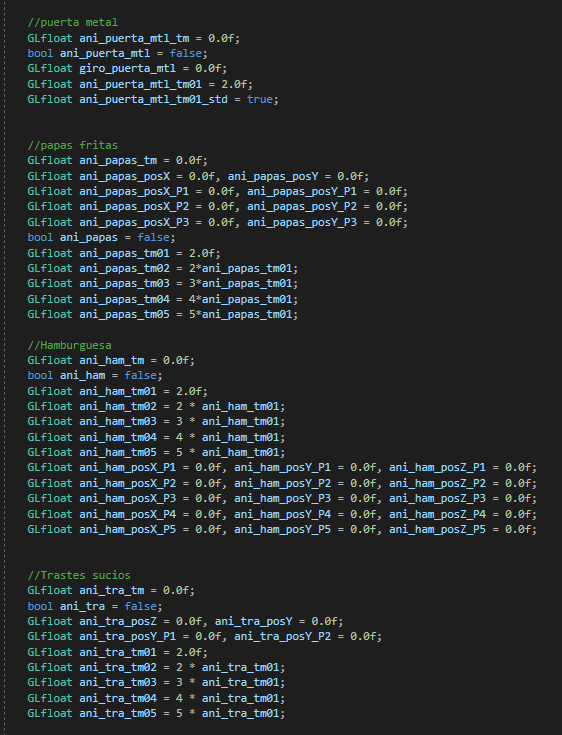
\includegraphics[scale=1]{img/img6}
		\centering
		\caption{Codigo}
	\end{figure}
\begin{figure}[H]
		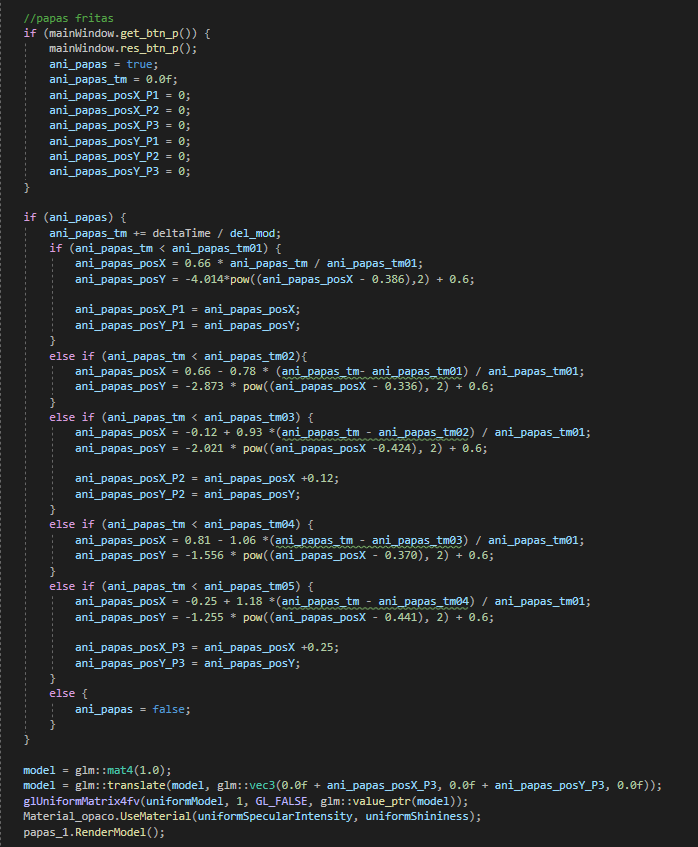
\includegraphics[scale=1]{img/img7}
		\centering
		\caption{Codigo}
	\end{figure}

Cada animación se realizo de manera independiente, es decir se pueden ejecutar todas las animaciones al mismo tiempo, para cada animación, se crearon funciones específicas para el movimiento espacial de los objetos, y es posible modificar los intervalos de cada animación o velocidad, aunque no es recomendable ya que los sonidos de algunas animaciones están al tiempo en que están corren.

\subsection{Luces}
\begin{figure}[H]
		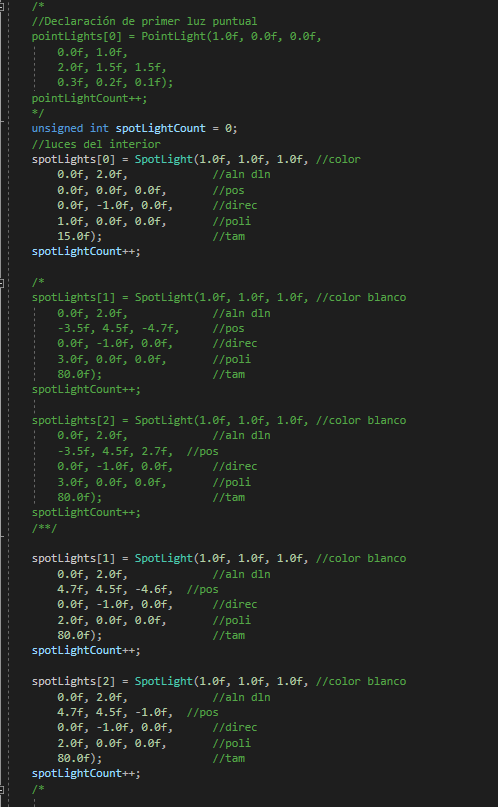
\includegraphics[scale=0.7]{img/img8}
		\centering
		\caption{Codigo}
	\end{figure}

Todas las luces son SpotLight, todas tiene dirección hacia abajo $-Y$, se cambiaron algunos parámetros para que funcionaran como focos, y se posicionaron el lugar correcto, para ello se crearon bases color negro el techo de la estructura donde están las luces.

\subsection{Sonido}
\begin{figure}[H]
		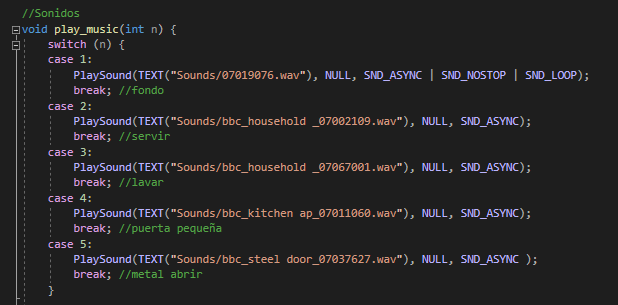
\includegraphics[scale=1]{img/img10}
		\centering
		\caption{Codigo}
	\end{figure}
\begin{figure}[H]
		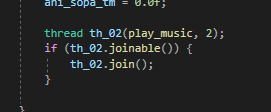
\includegraphics[scale=1]{img/img9}
		\centering
		\caption{Codigo}
	\end{figure}

Para el sonido se uso una biblioteca para reproducir sonido, no fue posible logra que varios sonidos se reproducen al mismo tiempo por lo que cuando se ejecuta una animación con sonido el sonido de fondo se detiene y al terminar vuelve a comenzar.

Por último, también fueron usados hilos, ya que ahora existe un hilo independiente del principal que ejecuta el sonido.

\newpage
\section{Resultado}

\end{document}

	\begin{figure}[H]
		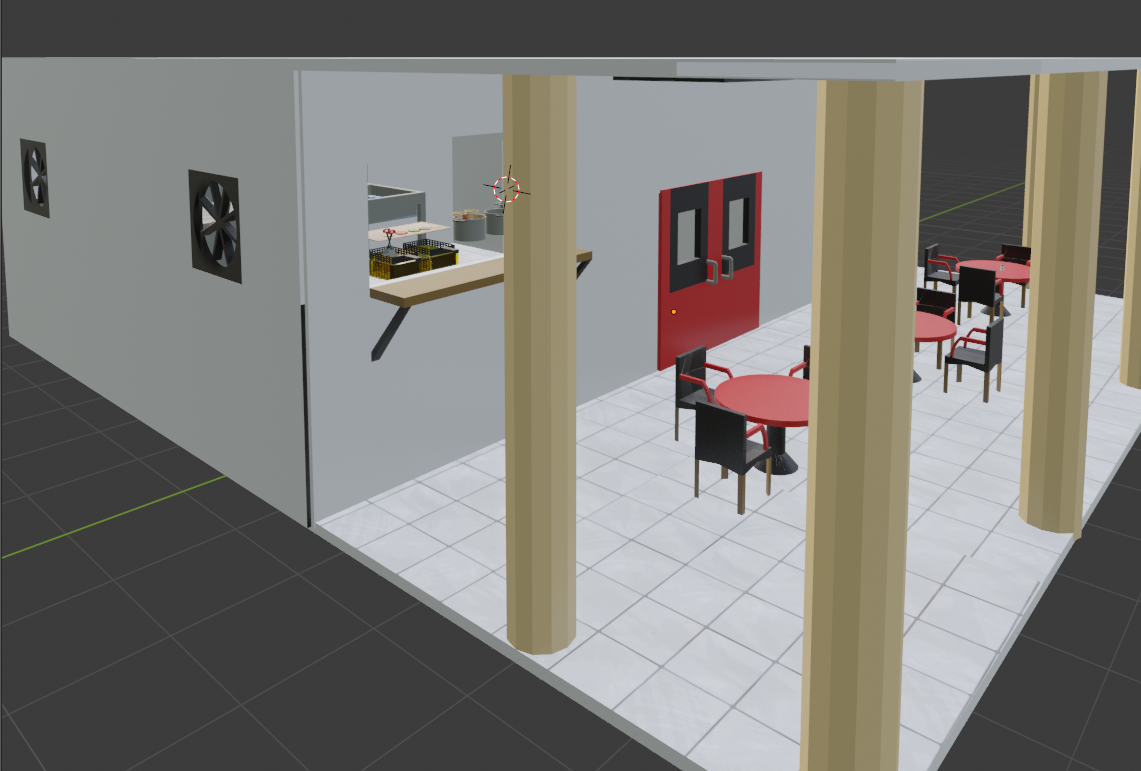
\includegraphics[scale=1]{img/img1}
		\centering
		\caption{Diagrama simulado en Multisim}
	\end{figure}

	\begin{figure}[H]
	 \centering
	  \subfloat[Osciloscopio]{
	    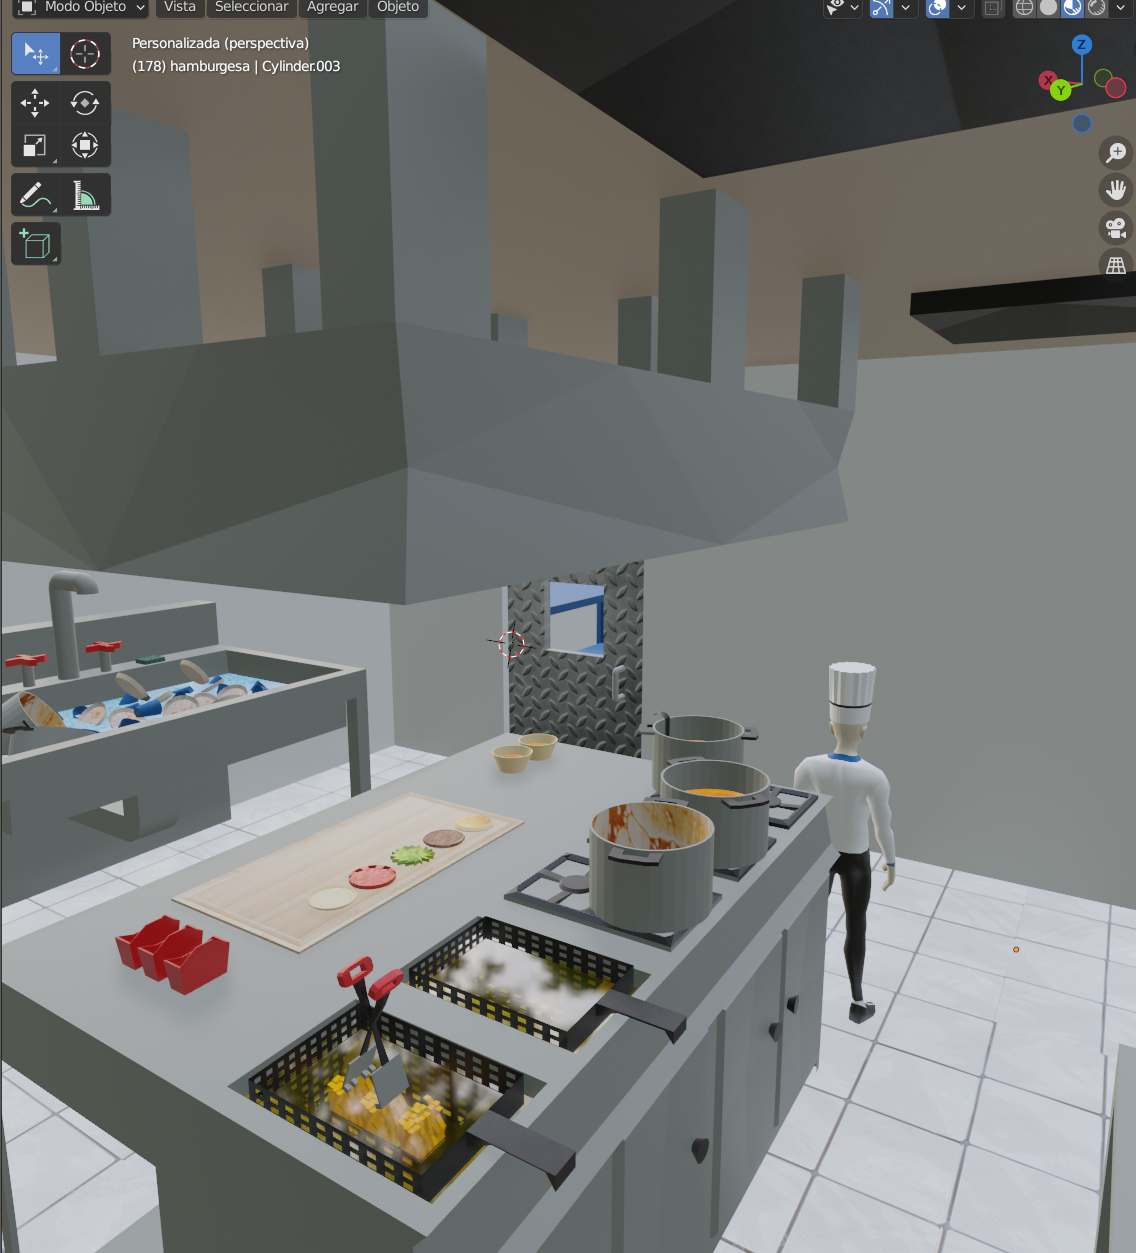
\includegraphics[width=0.45\textwidth]{img/img2}}
	  \subfloat[Analizador de espectro]{
	    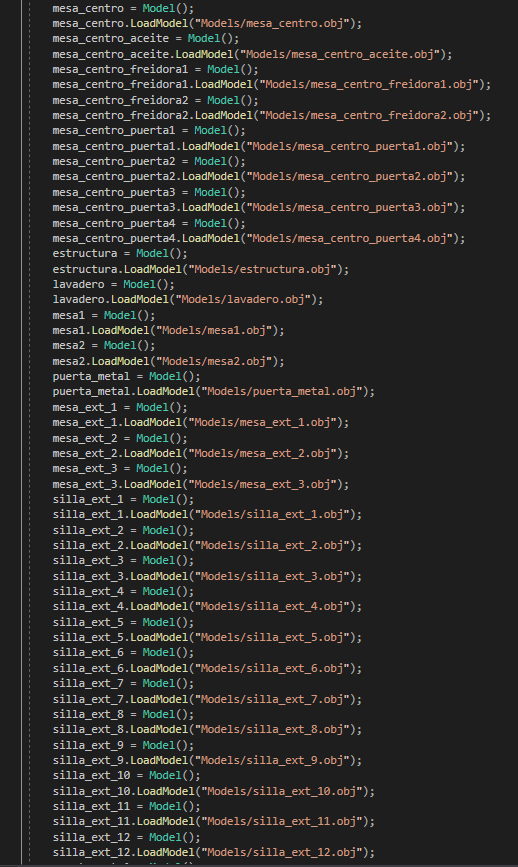
\includegraphics[width=0.45\textwidth]{img/img3}}
	 \caption{Salidas obtenidas}
	\end{figure}
